\subsection{Time and Space Analysis}
In this section, we evaluate both time and space improvements of each optimization on each query. We consider both before and after \emph{disk cache}. Moreover, the space improvement is considering the total size of the transferred tables between memory and disk. Execution time is measured in \emph{seconds}. \\

\begin{tabularx}{\textwidth}{|*{7}{Y|}}
\hline
\multirow{2}{*}{Query 1} 
  &\multicolumn{3}{c|}{Before Cache}&\multicolumn{3}{c|}{After Cache}\\
\cline{2-7}
  &Time &Time \% &Space \% &Time &Time \% &Space \% \\
\hline
Initial Query &16.78 &- &- &1.77 &- &- \\
\hline
After Index Opt. &- &- &- &- &- &- \\
\hline
After Query Opt. &10.87 &- &- &0.39 &- &- \\
\hline
After Schema Opt. &8.8 &- &- &0.33 &- &- \\
\hline
After Memory Opt. &7.8 &- &- &0.3 &- &- \\
\hline
\end{tabularx}

\begin{tabularx}{\textwidth}{|*{7}{Y|}}
\hline
\multirow{2}{*}{Query 2} 
  &\multicolumn{3}{c|}{Before Cache}&\multicolumn{3}{c|}{After Cache}\\
\cline{2-7}
  &Time &Time \% &Space \% &Time &Time \% &Space \% \\
\hline
Initial Query &1535 &- &- &1463 &- &- \\
\hline
After Index Opt. &9.49 &- &- &0.78 &- &- \\
\hline
After Query Opt. &7.75 &- &- &0.68 &- &- \\
\hline
After Schema Opt. &6.8 &- &- &0.65 &- &- \\
\hline
After Memory Opt. &5.77 &- &- &0.65 &- &- \\
\hline
\end{tabularx}

\begin{tabularx}{\textwidth}{|*{7}{Y|}}
\hline
\multirow{2}{*}{Query 3} 
  &\multicolumn{3}{c|}{Before Cache}&\multicolumn{3}{c|}{After Cache}\\
\cline{2-7}
  &Time &Time \% &Space \% &Time &Time \% &Space \% \\
\hline
Initial Query &0.36 &- &- &0.07 &- &- \\
\hline
After Index Opt. &0.23 &- &- &0.01 &- &- \\
\hline
After Query Opt. &0.19 &- &- &0.01 &- &- \\
\hline
After Schema Opt. &0.14 &- &- &0 &- &- \\
\hline
After Memory Opt. &0.12 &- &- &0 &- &- \\
\hline
\end{tabularx}

\begin{tabularx}{\textwidth}{|*{7}{Y|}}
\hline
\multirow{2}{*}{Query 4} 
  &\multicolumn{3}{c|}{Before Cache}&\multicolumn{3}{c|}{After Cache}\\
\cline{2-7}
  &Time &Time \% &Space \% &Time &Time \% &Space \% \\
\hline
Initial Query &10.41 &- &- &0.27 &- &- \\
\hline
After Index Opt. &- &- &- &- &- &- \\
\hline
After Query Opt. &- &- &- &- &- &- \\
\hline
After Schema Opt. &6.37 &- &- &0.15 &- &- \\
\hline
After Memory Opt. &6.01 &- &- &0.13 &- &- \\
\hline
\end{tabularx}

\begin{tabularx}{\textwidth}{|*{7}{Y|}}
\hline
\multirow{2}{*}{Query 5} 
  &\multicolumn{3}{c|}{Before Cache}&\multicolumn{3}{c|}{After Cache}\\
\cline{2-7}
  &Time &Time \% &Space \% &Time &Time \% &Space \% \\
\hline
Initial Query &6.14 &- &- &0.33 &- &- \\
\hline
After Index Opt. &- &- &- &- &- &- \\
\hline
After Query Opt. &4.39 &- &- &0.26 &- &- \\
\hline
After Schema Opt. &2.94 &- &- &0.21 &- &- \\
\hline
After Memory Opt. &2.34 &- &- &0.2 &- &- \\
\hline
\end{tabularx}

\subsection{Database Size Effect}
The following plots show the effect of increasing database sizes on the execution time of our $5$ queries. We consider both before and after \emph{disk cache}.

\begin{figure}[H]
    \centering
    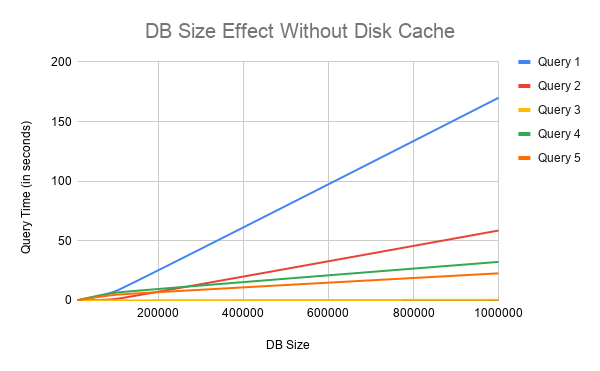
\includegraphics[width=0.8\textwidth]{images/db-size-without-cache.png}
    \caption{Database Size Effect Without OS (Disk) Cache.}
    \label{fig:db-size-1}
\end{figure}

\begin{figure}[H]
    \centering
    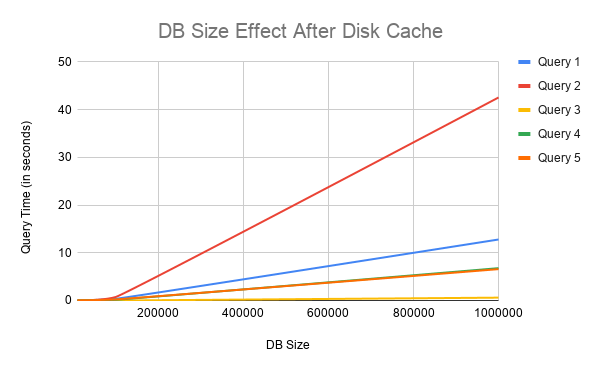
\includegraphics[width=0.8\textwidth]{images/db-size-after-cache .png}
    \caption{Database Size Effect After OS (Disk) Cache.}
    \label{fig:db-size-2}
\end{figure}

\subsection{Optimized SQL vs. NoSQL}

\subsection{Hardware Effect}
